
\section{Additional Experimental Results}
\subsection{Bayesian Neural Network Regression}\label{section:bnn_additional}

\begin{figure}[H]
  \centering
%%   \subfloat[Wine]{
%%     \includegraphics[scale=0.9]{figures/wine_04.pdf}
%%   }\hspace{0.2in}
  \subfloat[Concrete]{
    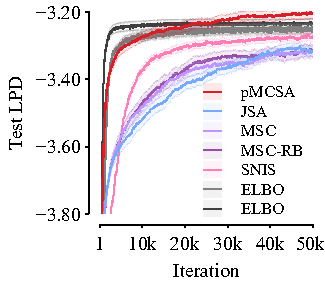
\includegraphics[scale=0.9]{figures/concrete_01.pdf}
  }\vspace{0.05in}\\
  \subfloat[Boston]{
    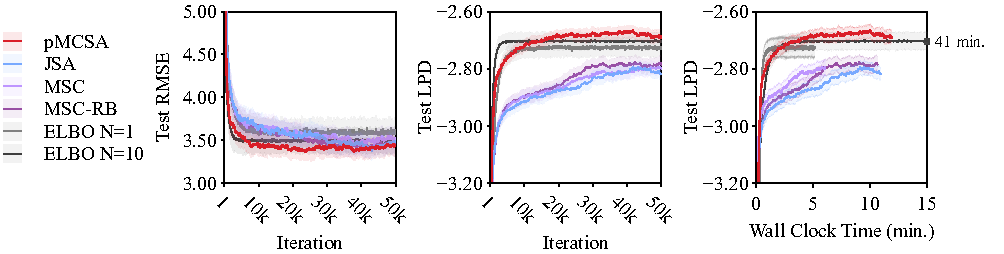
\includegraphics[scale=0.9]{figures/boston_01.pdf}
  }\vspace{0.05in}\\
  \subfloat[Yacht]{
    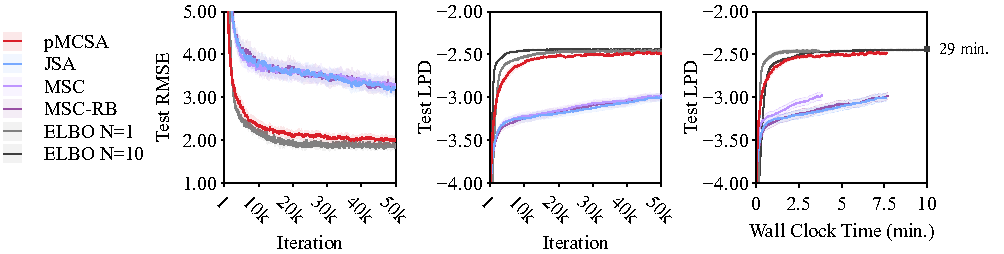
\includegraphics[scale=0.9]{figures/yacht_01.pdf}
  }\vspace{0.05in}\\
  \subfloat[Airfoil]{
    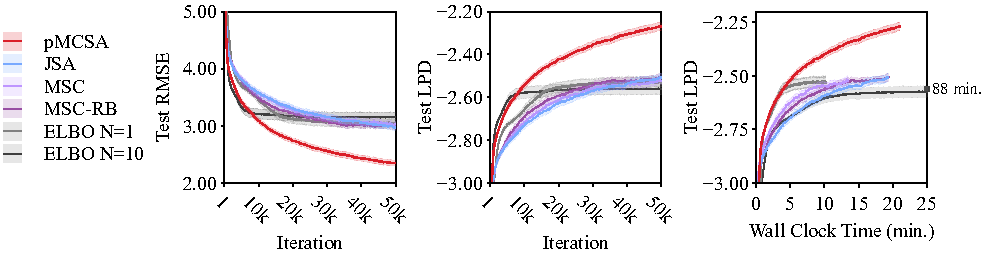
\includegraphics[scale=0.9]{figures/airfoil_01.pdf}
  }
  \caption{\textbf{Test root-mean-square error (RMSE) and test log predictive density (LPD) on Bayesian neural network regression.} 
    The grey squares mark the performance of ELBO \(N=10\) at the wall clock time shown next to it.
  The error bands show the 95\% bootstrap confidence intervals obtained from 20 independent 90\% train-test splits.}
\end{figure}

\begin{figure}[H]
  \centering
  \subfloat[Gas]{
    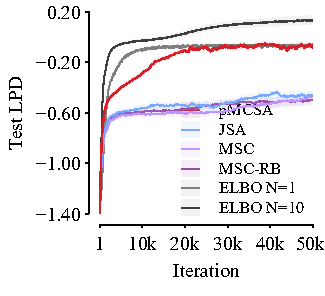
\includegraphics[scale=0.9]{figures/gas_01.pdf}
  }\vspace{0.05in}\\
  \subfloat[Energy]{
    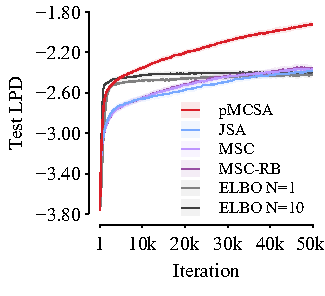
\includegraphics[scale=0.9]{figures/energy_01.pdf}
  }\vspace{0.05in}\\
  \subfloat[SML]{
    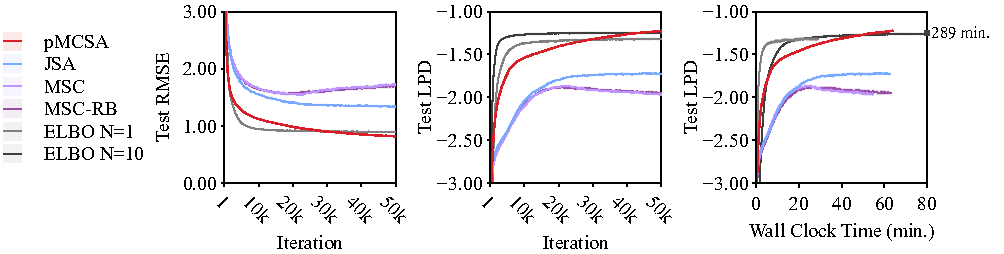
\includegraphics[scale=0.9]{figures/sml_01.pdf}
  }
  \caption{\textbf{(continued) Test root-mean-square error (RMSE) and test log predictive density (LPD) on Bayesian neural network regression.}
    The grey squares mark the performance of ELBO \(N=10\) at the wall clock time shown next to it.
  The error bands show the 95\% bootstrap confidence intervals obtained from 20 independent 90\% train-test splits.}
\end{figure}

\subsection{Robust Gaussian Process Regression}\label{section:gp_additional}
\begin{figure}[H]
  \centering
  \subfloat[Wine]{
    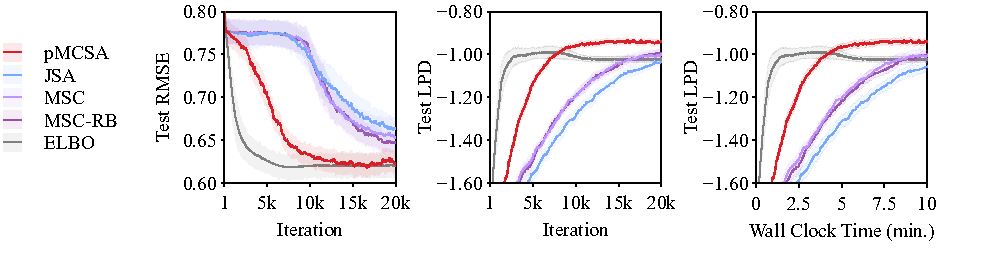
\includegraphics[scale=0.9]{figures/wine_pgp_01.pdf}
  } 
  \caption{\textbf{Test root-mean-square error (RMSE) and test log predictive density (LPD) on Robust Gaussian Process Regression.}
  The error bands shows the 95\% bootstrap confidence interval obtained from 20 repetitions.}
\end{figure}

\begin{figure}[H]
  \subfloat[Concrete]{
    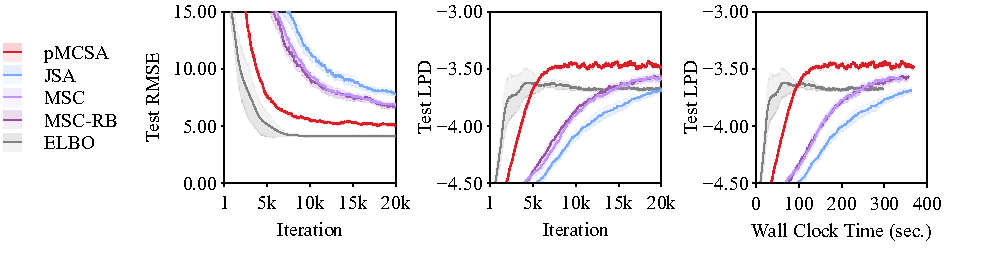
\includegraphics[scale=0.9]{figures/concrete_pgp_01.pdf}
  }\vspace{0.05in}\\
  \subfloat[Yacht]{
    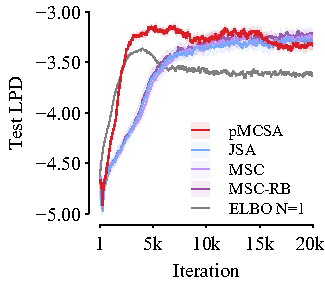
\includegraphics[scale=0.9]{figures/yacht_pgp_01.pdf}
  }\vspace{0.05in}\\
  \subfloat[Airfoil]{
    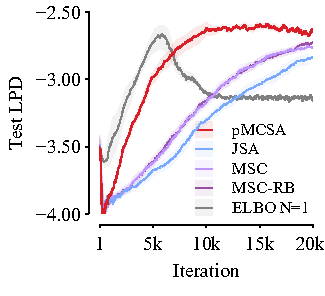
\includegraphics[scale=0.9]{figures/airfoil_pgp_01.pdf}
  }\vspace{0.05in}\\
  \subfloat[Energy]{
    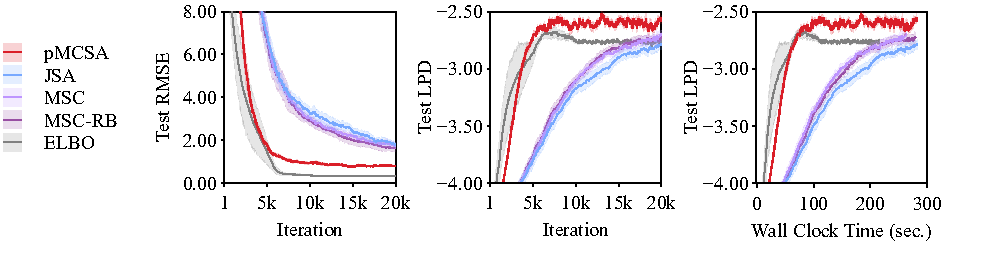
\includegraphics[scale=0.9]{figures/energy_pgp_01.pdf}
  } 
  \caption{\textbf{(continued) Test root-mean-square error (RMSE) and test log predictive density (LPD) on Robust Gaussian Process Regression.}
  The error bands show the 95\% bootstrap confidence intervals obtained from 20 independent 90\% train-test splits.
  }
\end{figure}

%%% Local Variables:
%%% TeX-master: "master"
%%% End:
